\chapter{\IfLanguageName{dutch}{Stand van zaken}{State of the art}}
\label{ch:stand-van-zaken}

% Tip: Begin elk hoofdstuk met een paragraaf inleiding die beschrijft hoe
% dit hoofdstuk past binnen het geheel van de bachelorproef. Geef in het
% bijzonder aan wat de link is met het vorige en volgende hoofdstuk.

% Pas na deze inleidende paragraaf komt de eerste sectiehoofding.
Dit overzicht biedt inzicht in de huidige stand van zaken en vormt de basis voor een weloverwogen keuze bij de ontwikkeling van een Proof of Concept (PoC). Dit betreft zowel de technische als de juridische aspecten. Daarnaast wordt in dit deel ook stilgestaan bij het belang van een vlot supportproces binnen IT.

Concreet komen de volgende onderwerpen aan bod:
\begin{itemize}
    \item \textbf{IT-support chatbot} - Wat zijn de mogelijkheden van om een IT-support chatbot te maken aan de hand van een {Large Language Models} (LLM) en welke factoren moeten in overweging worden genomen?
    \item \textbf{De AI Act en de belangrijkste richtlijnen} - Een overzicht van de relevante wet- en regelgeving en de impact hiervan op RAG-toepassingen.
    \item \textbf{Best practices voor IT-supportprocessen} - Inzichten in hoe RAG kan worden toegepast binnen IT-support en welke methodologieën het best kunnen worden gevolgd.
\end{itemize}

\section{IT-support chatbot}
    
    Om een IT-support chatbot te ontwikkelen, moeten verschillende aspecten in overweging worden genomen. Bij het gebruik van een LLM-model zijn er twee belangrijke opties: Retrieval-Augmented Generation (RAG) en Cache-Augmented Generation (CAG). Beide methoden maken gebruik van een LLM en verrijken de kennis van dit model met behulp van eigen documenten. Echter, beide benaderingen hebben specifieke voor- en nadelen. Het is daarom essentieel om deze zorgvuldig af te wegen om een weloverwogen keuze te maken voor een Proof of Concept (PoC).
    
    \subsection{Large Language Model}
    
    %TODO hier moet je veel uitgebreider over praten behandel ook onderwerpen zoals NLP en LM om dan naar dit punt te komen. Zal vollediger zijn en je kan op die manier ook veel meer tekst hebben
    
    WORK IN PROGRESS
    
     Een LLM is een geavanceerd neuraal netwerk dat getraind is op grote hoeveelheden tekstdata om menselijke taal te kunnen begrijpen, genereren en manipuleren. LLM's gebruiken de transformer architectuur, zoals geïntroduceerd door \textcite{Vaswani2017}, die uitblinkt in het modelleren van sequentiële tekst en contextuele afhankelijkheden.
      
     Deze modellen worden "large" genoemd vanwege hun schaal: ze bevatten vaak miljarden parameters. Getraind door op gigantische bronnen aan data, kunnen LLM's tekst genereren die coherente, contextuele en soms zelfs creatieve eigenschappen vertoont \cite{Gupta2025}.
      
     Toepassingen van LLM's omvatten onder andere chatbots, automatische vertaling, samenvatten van documenten, codegeneratie, en vragen-beantwoording. Hoewel hun prestaties indrukwekkend zijn, bestaan er ook zorgen over bias, hallucinatie van onjuiste informatie, en het gebruik van niet-gecontroleerde trainingsdata \cite{Gupta2025}.
      
     De ontwikkeling van LLM’s markeert een belangrijke stap richting algemene taalintelligentie, maar roept tegelijkertijd vragen op over ethiek, transparantie, en betrouwbaarheid in gebruik \cite{Gupta2025}.
     
    \subsection{Retrieval Augmented Generation}
    
    LLM's hebben de afgelopen jaren een enorme opmars gemaakt en vandaag de dag hebben deze modellen een brede impact op verschillende domeinen in de samenleving. Ondanks hun indrukwekkende mogelijkheden brengen LLM’s ook enkele nadelen met zich mee. Zo kunnen ze hallucineren, beschikken ze niet altijd over de meest actuele informatie, en missen ze vaak domein- en bedrijfsspecifieke kennis.  
    
    Een mogelijke oplossing voor deze beperkingen is \textit{Retrieval-Augmented Generation} (RAG). Deze techniek combineert de kracht van LLM’s met externe databronnen om nauwkeurigere en beter onderbouwde antwoorden te genereren. In deze sectie wordt toegelicht wat RAG is, hoe het werkt en op welke manier het kan bijdragen aan de ontwikkeling van een effectieve support chatbot.
    
    \subsubsection{Wat is RAG}
    RAG, oftewel Retrieval-Augmented Generation, is een techniek die, zoals eerder vermeld, een oplossing biedt voor de tekortkomingen van klassieke LLM’s. Door externe databronnen te gebruiken, kan een traditioneel LLM-model betere resultaten behalen. Deze methode maakt het mogelijk om domeinspecifieke data te integreren en modellen bij te werken met actuele informatie. Zo kunnen klassieke LLM’s worden verrijkt met nieuwe, up-to-date gegevens die voldoen aan specifieke behoeften \autocite{Wu2024}.
    
    Om RAG in de praktijk toe te passen, moeten een aantal stappen worden doorlopen. Deze worden in het volgende deel nader toegelicht, maar samengevat bestaat het proces uit de volgende fasen:
    
    \begin{enumerate}
        \item {Ophalen}
        \item {Verrijking}
        \item {Generatie}
    \end{enumerate}
    
    \subsubsection{Hoe werkt RAG}
    
    Het doel van RAG is om een LLM te verrijken met specifieke kennis, zodat de gebruiker beter ondersteund wordt bij het beantwoorden van gerichte vragen. Dit proces bestaat uit drie hoofdfasen. Eerst wordt relevante informatie opgehaald (Retrieval). Vervolgens wordt het antwoord verrijkt op basis van de beschikbare documentatie. Tot slot genereert de LLM een antwoord op de gestelde vraag.
    
    Op Figuur \ref{fig:Rag process} is te zien die dit proces illustreert.
    
    \begin{figure}[H]
        \centering
        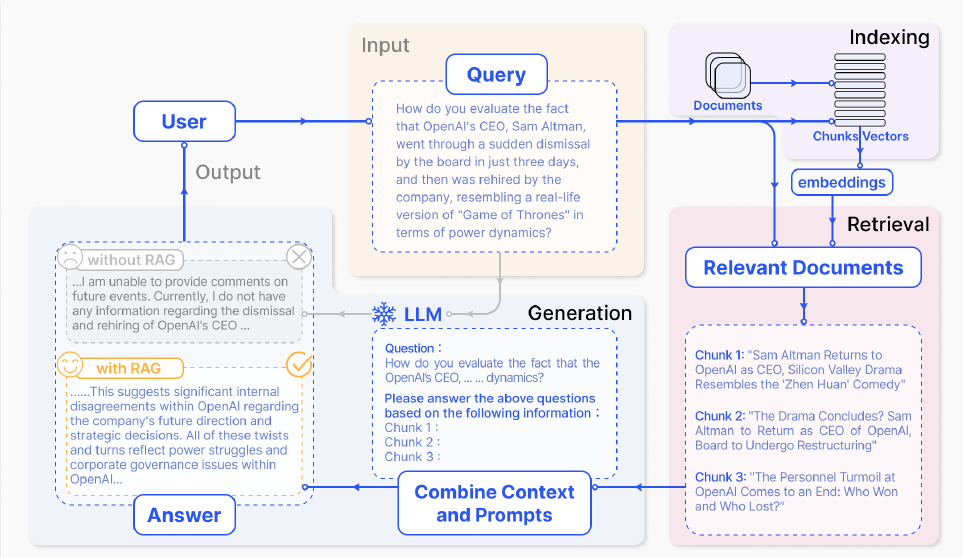
\includegraphics[width=\textwidth]{RagGao2023.png}
        \caption{Een generieke RAG architectuur \cite{Gao2023}}
        \label{fig:Rag process}
    \end{figure}
    
    \paragraph{Ophalen}
     
    Voordat een LLM effectief ondervraagd kan worden met informatie die via documentverrijking is toegevoegd, moet eerst een grondige voorbereidende verwerking plaatsvinden. Dit proces omvat het selecteren van relevante documenten en het vervolgens combineren van deze informatie met de gestelde vraag. Deze vraag en de geselecteerde documentfragmenten, die worden opgehaald vanuit de vector database, worden toegevoegd aan de context van de de LLM die vervolgens in staat is om een contextueel passend antwoord te genereren.
    
    Een eerste essentiële stap in dit proces is het identificeren en selecteren van de documenten die inhoudelijk relevant zijn voor de vraagstelling. Deze documenten worden niet in hun geheel, maar in kleinere segmenten verwerkt, zogenaamde "chunks". Het opdelen in chunks is noodzakelijk omdat volledige documenten doorgaans te omvangrijk zijn om efficiënt te verwerken binnen de contextlimieten van een LLM. Bovendien maakt deze fragmentatie het mogelijk om op een meer gerichte manier informatie te extraheren uit de vector database \autocite{Wu2024}.
    
    Voor het opdelen van documenten bestaan verschillende methodologische benaderingen. Een veelgebruikte techniek is het verdelen van tekst op basis van een vooraf bepaald aantal tokens of karakters, zodat elke chunk ongeveer dezelfde lengte heeft. Een alternatieve strategie, die vooral geschikt is voor natuurlijke taalteksten, is het opdelen op basis van zinnen of alinea’s. Deze aanpak draagt doorgaans bij aan het behoud van de semantische samenhang binnen een chunk, wat de kwaliteit van de informatieophaling ten goede komt \autocite{Wang2024}.
    
    Na het opdelen worden deze tekstsegmenten omgezet in zogeheten embeddings. Dit zijn vector representaties die de semantische inhoud van de chunks op een wiskundige manier vastleggen. Deze embeddings worden vervolgens opgeslagen in een vector database, een specifiek type gegevensopslag dat geoptimaliseerd is voor het bewaren en efficiënt ophalen van vectorrepresentaties op basis van semantische gelijkenis \autocite{Wu2024}. Dit gehele proces vormt de basis waarop de LLM tijdens het beantwoorden van vragen relevante context uit de vector database kan ophalen en verwerken.
   
     \begin{figure}[H]
        \centering
        \includegraphics[width=\textwidth]{retrieverWu2024.png}
        \caption{Documentverwerking en opslag in een vector database via embeddings \cite{Wu2024}}
        \label{fig:RAG opmaken vector database}
    \end{figure}
    
    Zodra de documenten via embeddings zijn toegevoegd aan de vector database, zal een gebruiker in de context van RAG (Retrieval-Augmented Generation) ook vragen stellen. Een vraag of query wordt, net als de documenten, vertaald naar embeddings. Op basis van deze embeddings worden de top-k dichtstbijzijnde buren uit de vector database opgehaald. Dit betekent dat de meest relevante delen van de opgeslagen documenten worden opgehaald. Deze relevante “chunks” worden vervolgens gebruikt om context te bieden aan het LLM-model dat wordt ondervraagd \autocite{Wu2024}.
    
            
    \begin{figure}[H]
        \centering
        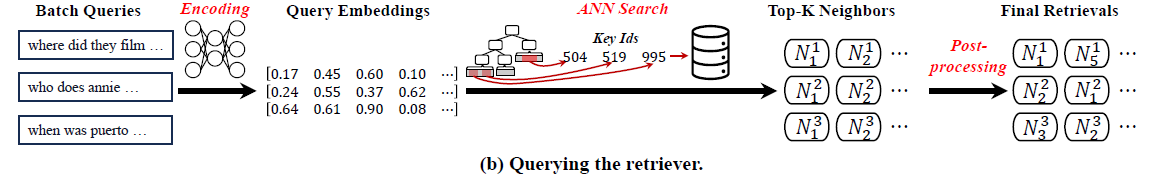
\includegraphics[width=\textwidth]{QueryRetrieverWu2024.png}
        \caption{Vraagafhandeling en ophalen van relevante chunks \cite{Wu2024}}
        \label{fig:RAG bevragen vector database}
    \end{figure}
    
    \paragraph{Generatie}
    
    Zodra de meest relevante informatie is opgehaald, wordt deze gebruikt in het proces. Uiteindelijk blijft het de bedoeling om het LLM-model te bevragen. De opgehaalde documenten worden, samen met de vraag van de gebruiker, toegevoegd aan de context van het model. Hierdoor beschikt het LLM-model over extra informatie en kan het deze verwerken. Dit leidt tot een antwoord voor de gebruiker, gebaseerd op de geïnjecteerde kennis \autocite{Zhao2024}.
    
    \subsection{Cache-Augmented Generation}
    
    Met de opkomst van nieuwe LLM modellen die een grotere context bevatten is het niet altijd nodig om te werken met een RAG architectuur. Wanneer het aantal documenten en de lengte ervan niet dermate groot is kan je ook meteen alle documenten injecteren in de context van een LLM model. Dit zorgt voor een heel simpele en efficiënte benadering om een LLM model bedrijf- of contextspecifieke kennis te geven.
    
    \subsection{RAG vs CAG}
    
    
    \subsection{LLM benchmarks}
    Om te bepalen welke modellen het meest geschikt zijn voor de ontwikkeling van IT-support chatbot, is een objectieve meetmethode noodzakelijk. Gelukkig bestaan er verschillende platformen die LLM's vergelijken en rangschikken op basis van prestaties. In deze sectie bespreken we enkele van deze platformen en maken we een selectie van modellen die het meest geschikt lijken voor het bouwen van een RAG-model.
       
    \paragraph{LiveBench} 
    Een platform dat LLM-modellen evalueert, is LiveBench. Dit platform stelt een rangschikking op voor verschillende modellen en biedt een actuele scorebord die elke zes maanden wordt bijgewerkt. Voor deze bachelorproef zal gebruik worden gemaakt van de ranking afkomstig uit november 2024.
    
    LiveBench beoordeelt LLM-modellen op basis van zes categorieën. Binnen elke categorie worden meerdere taken uitgevoerd om een nauwkeurige beoordeling te verkrijgen. De zes categorieën zijn:
    \begin{itemize}
        \item Wiskundige vaardigheden (Math)
        \item Programmeervaardigheden (Coding)
        \item Redeneren en probleemoplossing (Reasoning)
        \item Data-analyse (Data Analysis)
        \item Volgen van instructies (Instruction Following)
        \item Begrip van natuurlijke taal (Language Comprehension)
    \end{itemize}
    
    Elke categorie wordt geëvalueerd op basis van specifieke taken. Dit resulteert uiteindelijk in een algemene rangschikking, waarin zowel de beste modellen per categorie als het beste presterende model overall worden geïdentificeerd.
    
    \begin{figure}[H]
        \centering
        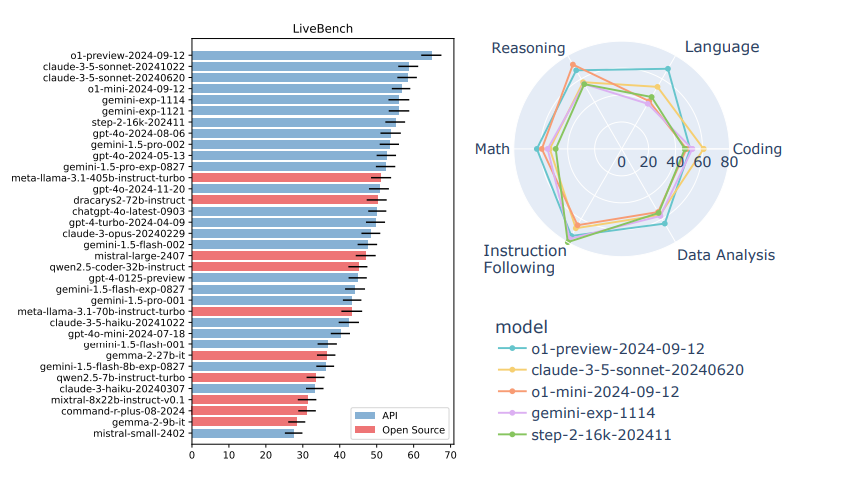
\includegraphics[width=\textwidth]{LiveBenchRanking.png}
        \caption{LiveBench ranking van verschillende LLMs.}
        \label{fig:livebench}
    \end{figure}
    
    Uit de ranking van LiveBench kan geconcludeerd worden dat 3 verschillende organisaties elk een model aanbieden die vanuit globaal oogpunt tot de top 3 behoort. Deze top 3 zijn: 
    \begin{enumerate}
        \item claude-3-5-sonnet-20240620 van Anthropic
        \item Meta-llama-3.1-405b-instruct-turbo van Meta
        \item gpt-4o-2024-05-13 van OpenAI
    \end{enumerate}
    
    \subsubsection{Chatbot arena} 
    
    Een andere benchmark tool Chatbot arena, net zoals LiveBench is Chatbot arena een site die een actuele weergave biedt van de beste LLM's op basis van vooraf gedefinieerde categorieën. 
    Volgens de ranking van \textcite{LiveBench2025} zijn dit de top 3 LLM's:
    
    \begin{enumerate}
        \item GPT-4-Turbo van OpenAI
        \item GPT-4-0613 van OpenAI
        \item Mistral-Medium Mistral AI
    \end{enumerate}
    
    Hoewel het doel van beide benchmarks hetzelfde is is de manier van werken wel anders. ChatbotArena gaat gebruikers twee anonieme LLM modellen tegenover elkaar plaatsen, de gebruiker kan vervolgens een eigen vraag stellen en de gebruiker bepaalt zelf welke van de 2 het beste resultaat heeft opgeleverd.
    
    Het voordeel van deze methode is dat de LLM-modellen realistische cases moeten behandelen die door gebruikers zelf worden gesteld. Op basis van resultaten die de LLM modellen tonen kan een gebruiker zijn voorkeur meegeven. Het nadeel van deze manier van werken is dat de gebruikers die deze testen uitvoeren niet representatief zijn voor alle gebruikers van LLM-modellen. De gebruikers die deze testen uitvoeren zijn vaak mensen met een interesse in LLM-modellen of mensen die onderzoek doen in dit vakgebied. Desondanks kan op basis van deze stemmen verscheidene modellen tegenover elkaar worden geplaatst. In januari 2024 werden ruim 240.000 stemmen uitgebracht door ongeveer 90.000 gebruikers \autocite{Chiang2024}. 
    
    \paragraph{Conclusie}
    
    %TODO Navragen of ze een lijst van criteria hebben welke LLM wel en niet te gebruiken => geen echte beperkingen inzake LLM maar zou best moeten kunnen draaien op Azure opgeving dus chatGPT zou hierbij zeker de voorkeur hebben.
    Op basis van de 2 benchmarks die hier werden besproken kan niet meteen éénduidig besloten worden welke modellen het best zouden gebruikt worden voor het maken van het RAG model. Aangezien dit een zeer volatiele omgeving is met veel en snelle ontwikkelingen zijn de modellen die vandaag het beste scoren over een maand potentieel voorbij gestoken door nieuwe modellen. Desalniettemin bevatten deze benchmarks heel wat nuttige informatie en inzichten over de sterktes van bepaalde modellen tegenover andere modellen. 
    
    \subsection{Evaluatiemethoden voor LLM-output}
   
    Het gebruik van een performante LLM volstaat op zich niet. Minstens even belangrijk is het evalueren van de kwaliteit en accuraatheid van de gegenereerde antwoorden. Hiervoor bestaan verschillende evaluatiemethoden, waaronder de Bilingual Evaluation Understudy (BLEU), de Recall-Oriented Understudy for Gisting Evaluation (ROUGE), en BERTScore.  
    
    Deze methoden kennen elk hun eigen berekeningswijze, maar delen een belangrijk gemeenschappelijk kenmerk. Ze zijn allen afhankelijk van de aanwezigheid van een referentie-antwoord. Dit referentie-antwoord wordt gebruikt als maatstaf om de gegenereerde output van de LLM mee te vergelijken en zo een score toe te kennen die de kwaliteit van de output reflecteert \cite{microsoft2024evaluation}.
    
    \paragraph{BLEU Score}
    
    De BLEU score is een evaluatie metriek die oorspronkelijk werd ontwikkeld om de kwaliteit van door machines gegenereerde vertalingen te beoordelen. Hierbij wordt de output van het model vergeleken met een of meerdere menselijke referentievertalingen. Aan de hand van overlappingen of zogenaamde n-gram overeenkomsten, reeksen van één of meerdere opeenvolgende woorden, wordt een score toegekend. De score ligt tussen 0 en 1, waarbij een hogere score duidt op een grotere overeenkomst met de referentietekst \cite{papineni-etal-2002-bleu}.
    
    Een score van 1 betekent een perfecte overeenkomst, maar zelfs menselijke vertalingen behalen zelden deze score, omdat er vaak meerdere correcte vertaalmogelijkheden bestaan die kunnen afwijken. Hoewel BLEU een snelle en reproduceerbare maat biedt voor evaluatie, heeft het beperkingen doordat het geen rekening houdt met betekenis en contextuele variatie \cite{papineni-etal-2002-bleu}.
    
    \paragraph{ROUGE Score}
    
    Net zoals de BLEU-score evalueert de ROUGE-score de mate van overlap tussen een door machine gegenereerde tekst en een menselijke referentie. Waar BLEU echter voornamelijk gericht is op de precisie van exacte n-gram overeenkomsten, focust ROUGE sterker op de inhoudelijke dekking van de referentie. Hierdoor biedt de ROUGE-score een diepgaander inzicht in de kwaliteit van het gegenereerde antwoord \cite{Ganesan2018}.
    
    \paragraph{BERTScore}

\section{De AI Act en de belangrijkste richtlijnen}
Wat houdt de AI Act in, en wat zijn de belangrijkste richtlijnen die hierin moeten worden gevolgd?

\section{Best practices voor IT-supportprocessen}
Wat zijn de bestaande best practices voor de organisatie van IT-supportprocessen?
